\documentclass[usenames,dvipsnames,notes,11pt,aspectratio=169,hyperref={colorlinks=true, linkcolor=blue}]{beamer}
\usepackage{ifthen}
\usepackage{xcolor}
\usepackage{pgfplots}
\usepackage{amsmath}
\usepackage{centernot}
\usepackage{pifont}
\usepackage{tabularx}
\usepackage{makecell}
\usepackage{cuted}
\usepackage{booktabs}
\usepackage{array}
\usepackage{textcomp}
\usepackage{setspace}
\usepackage{xspace}
\usepackage{subcaption}
\usepackage{tikz}
\usepackage{pdfcomment}
%\newcommand{\pdfnote}[1]{\marginnote{\pdfcomment[icon=note]{#1}}}
\newcommand{\pdfnote}[1]{}

\usepackage{pgfpages}
%\setbeameroption{show notes on second screen}


\input ../beamer-style
\input ../std-macros
\input ../macros

\newcommand{\pt}{\partial}

\AtBeginSection[]
{
    \begin{frame}
        \frametitle{Table of Contents}
        \tableofcontents[currentsection]
    \end{frame}
}
\parskip=10pt

\title[CSCI-GA.2590]{Pretraining and Finetuning}
\author[He He]{He He
}
\institute[NYU]{
    
\includegraphics[height=1cm]{../figures/nyu-logo}\\
}
\date{February 19, 2025}

\begin{document}
\begin{frame}
\titlepage
\end{frame}

\section{Review}

\begin{frame}
    {Last week}
    \begin{wideitemize}
        \item {\bf Encoders}: tokens to vectors
        \item {\bf Decoders}: vectors to tokens
        \item {\bf Key difference}: (autoregressive) decoders cannot look at the future
            \begin{itemize}
                \item Need causal masking
                \item Sequential output
            \end{itemize}
        \pause
        \item Can you use an encoder to generate tokens?\pause
        \item Can you use a decoder to encode text?
    \end{wideitemize}
\end{frame}

\section{Introduction}

\begin{frame}
    {Representation learning}
    Recap: What are good representations?\\
    \begin{itemize}
        \item Enable a notion of distance over text (word embeddings)
        \item Contains good features for downstream tasks 
    \end{itemize}

    \pause
    Examples:
        \begin{tabular}{ll}
            negative & the food is good but doesn't worth an hour wait
        \end{tabular}
    
    \vspace{-1em}
    \begin{itemize}
        \item Simple features (e.g. unigram BoW) require complex models.\\\pause
        \item \blue{Good features} only need \blue{simple models} (e.g. linear classifier) .
    \begin{figure}
        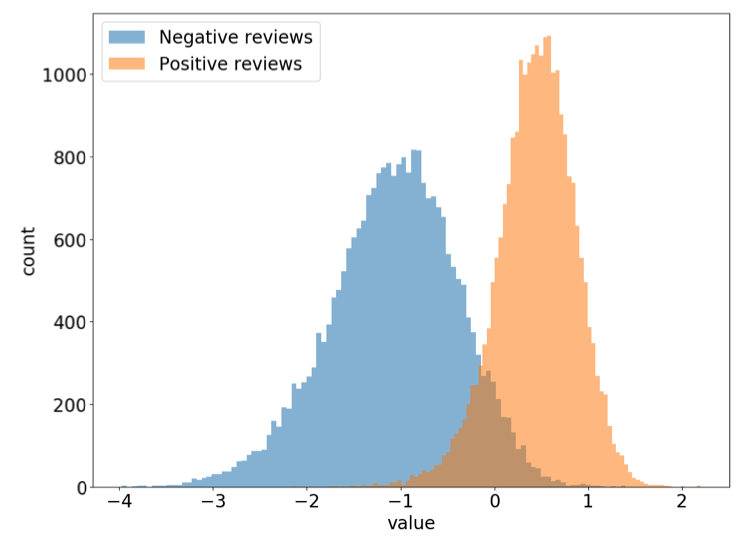
\includegraphics[height=3cm]{figures/sentiment}
        \caption{\href{https://arxiv.org/abs/1704.01444}{Sentiment neuron} [Radford et al., 2017]}
    \end{figure}
    \end{itemize}
\end{frame}

\begin{frame}
    {Representation learning}
    What can we do with good representations:\\
    \begin{itemize}
        \item Learning with small data: fine-tuning learned representations
        \item Transfer learning: one model/representation for many tasks 
        \item Metric learning: get a similarity metric
    \end{itemize}

    \pause\bigskip
    How to obtain such a representation:\\
    \begin{itemize}
        \item Training a neural network on any task gives us a representation good for \textit{that task}.
        \item But on which task can we learn good \textit{general} representations?
    \end{itemize}
\end{frame}

\begin{frame}
    {What can we learn from word prediction given context?}
    \begin{itemize}
        \itemsep1em
        \item The cats that are raised by my sister \rule{1.5cm}{0.5mm} sleeping. \pause\hfill \textit{syntax}
        \item Jane is happy that John invited \rule{1.5cm}{0.5mm} friends to his birthday party. \pause\hfill \textit{coreference}
        \item \rule{1.5cm}{0.5mm} is the capital of Tanzania. \pause\hfill \textit{knowledge}
        \item The boy is \rule{1.5cm}{0.5mm} because he lost his keys.  \pause\hfill \textit{commonsense}
        \item John took 100 bucks to Vegas. He won 50 and then lost 100. Now he only has \rule{1.5cm}{0.5mm} to go home. \pause\hfill \textit{numerical reasoning}
    \end{itemize}

    \pause\medskip
    Text contains a surprisingly large number of tasks!

    %\think{But aren't we already doing this in skip-gram / CBOW?}
\end{frame}

\begin{frame}
    {Self-supervised learning for representation learning}

    \textbf{Key idea}: predict parts of the input from the rest\\
    \begin{itemize}
        \item \blue{No additional supervision} is needed---both input and output are from the raw text data.
        \item Easy to \blue{scale}---massive amount of text on the Internet.
        \item Learned representation is \blue{general}---useful for any tasks that can be performed in textual mode.
    \end{itemize}
    \pause
    How is this different from skip-gram / CBOW?
    % want an encoder and/or decoder, not just word embeddings. No independence assumption.

    \pause
    \textbf{Approach}:\\
    \begin{itemize}
        \item \textbf{Pretrain}: train a model using self-supervised learning objectives on large data.
        \item \textbf{Finetune}: update part or all of the parameters of the pretrained model on labeled data of a downstream task.
    \end{itemize}
\end{frame}

\begin{frame}
    {A bit of history}
    \begin{itemize}[<+->]
        \item Pretrain an \blue{RNN} model on unlabeled data and finetune on supervised tasks
            \mycite[https://arxiv.org/pdf/1511.01432.pdf]{[Dai et al., 2015]}
            \mycite[https://arxiv.org/pdf/1511.01432.pdf]{[ULMFiT; Howard et al., 2018]}
            \begin{itemize}[<.->]
                \item Promising results on a small scale
            \end{itemize}
        \item ELMo: replace static word embedding by \blue{contextual word embeddings} from pretrained \blue{bi-LSTM} \mycite[https://arxiv.org/abs/1802.05365]{[Peters et al., 2018]}
            \begin{itemize}[<.->]
                \item First impactful result in NLP
            \end{itemize}
        \item Pretrain a \blue{Transformer} model and finetune on supervised tasks 
            \begin{itemize}[<.->]
                \item GPT \mycite[https://s3-us-west-2.amazonaws.com/openai-assets/research-covers/language-unsupervised/language_understanding_paper.pdf]{[Radford et al., 2018]},
                    BERT \mycite[https://arxiv.org/abs/1810.04805]{[Devlin et al., 2018]}
            \end{itemize}
        \item \blue{Scale} pretrained transformer to larger data and compute
            \begin{itemize}[<.->]
                \item Can directly answer user questions and solve many tasks, e.g., ChatGPT, Claude, Deepseek-chat
            \end{itemize}
    \end{itemize}
\end{frame}

\section{Tokenization}

\begin{frame}
    {Challenges in tokenization}
    We want to train models on all text on the internet. What are the challenges in tokenization? \pause
    \begin{wideitemize}
        \item A long tail of rare words\\
            \gray{Neologism, terminologies, misspelling, informal text, etc.}
        \item A mixture of multiple natural languages, programming languages, special symbols\\
            \gray{Low-resource language, math equations, code-switching, emoji, etc.}
        \item Efficiency\\
            \gray{Trade-off between vocab size and sequence length, latency}
    \end{wideitemize}
\end{frame}

\begin{frame}
    {Subword tokenization}
    The most widely adopted solution: decomposing words into subword units
    \begin{wideitemize}[<+->]
        \item A long tail of rare words\\
            \texttt{bioorthogonal} $\rightarrow$ {\tt bio \#\#ortho \#\#gonal}
        \item A mixture of multiple natural languages, programming languages, special symbols\\
            \texttt{Donaudampfschifffahrtsgesellschaft} $\rightarrow$ {\tt Donaudampf \#\#schiff \#\#fahrts \#\#gesellschaft} \gray{(German compound noun meaning "Danube steamship company")}
        \item Efficiency\\
            Balancing granularity and efficiency: reducing token count without losing meaning
    \end{wideitemize}
\end{frame}

\begin{frame}
    {Byte pair encoding (BPE)}

    What is a ``token''?\\
    \begin{itemize}
        \item A sequence of characters that carries some meaning and \blue{re-occurs} in a corpora
        \item Can we find these character units based on their \blue{frequency}?
    \end{itemize}

    \pause\medskip
    BPE:\\
    \begin{itemize}
        \item Origin: a \blue{compression algorithm} that iteratively replace the most common character sequences by a single symbol, e.g., {\tt un} $\rightarrow$ {\tt A}
            %\begin{itemize}
            %    \item Output: compressed text + a look-up table (to decompress)
            %\end{itemize}
        \item Start with individual characters as tokens
        \item Merge the most frequent pair of tokens and treat them as a single token
        \item Update the input with the new token and repeat the process
        \item Output: tokenized text and \blue{a set of merge rules}
    \end{itemize}
\end{frame}

\begin{frame}
\frametitle{BPE Example (Step-by-Step)}

\textbf{Initial Sequence:}\\
\begin{itemize}
    \item Words: \texttt{banana}, \texttt{band}, \texttt{ban}
    \item Initial tokenization (by character):
    \begin{itemize}
        \item \texttt{b a n a n a}
        \item \texttt{b a n d}
        \item \texttt{b a n}
    \end{itemize}
\end{itemize}

\pause
\textbf{Step 1: Count Pairs}\\
\begin{itemize}
    \item What is the most frequent pair: \pause\texttt{a n}
\end{itemize}

\pause
\textbf{Step 2: Merge}\\
\begin{itemize}
    \item New merge rule: {\tt a}, {\tt n} $\rightarrow$ \texttt{an}
    \item Updated tokenization:
    \begin{itemize}
        \item \texttt{b a n a n a} $\rightarrow$
        \item \texttt{b a n d} $\rightarrow$
        \item \texttt{b a n} $\rightarrow$
    \end{itemize}
\end{itemize}
\end{frame}

\begin{frame}
\frametitle{BPE Example (Step-by-Step)}

\textbf{Step 3: Count Pairs Again}\\
\begin{itemize}
    \item Updated tokenization:
    \begin{itemize}
        \item \texttt{b an an a}
        \item \texttt{b an d}
        \item \texttt{b an}
    \end{itemize}
    \item Most frequent pair: \texttt{b an}
\end{itemize}

\textbf{Step 4: Merge}\\
\begin{itemize}
    \item New merge rule: \texttt{b,  an} $\rightarrow$ \texttt{ban}
    \item Updated tokenization:
    \begin{itemize}
        \item \texttt{ban an a}
        \item \texttt{ban d}
        \item \texttt{ban}
    \end{itemize}
\end{itemize}
\end{frame}

%\begin{frame}
%    {BPE tokenization: inference}
%    Output from BPE tokenization:
%    \begin{itemize}
%        \item Tokenized (training) corpus
%        \item Ranked merge rules, e.g., \\
%            1. {\tt a}, {\tt n} $\rightarrow$ \texttt{an}\\
%            2. \texttt{b,  an} $\rightarrow$ \texttt{ban}
%    \end{itemize}
%\end{frame}

\begin{frame}
    {BPE: practicalities}
    \begin{wideitemize}
        \item Repeat the process until the desired number of merges or vocabulary size is reached (a hyperparameter to decide). Typically vocabulary sizes are 32-64K.
        \item Break ties deterministically, e.g., lexicographical order, occurrence in the corpus etc.
        \item Use bytes as the initial tokens (adopted by GPT-2)
        \item Variants: instead of merging the pair with the largest frequency, {\bf WordPiece} merges the pair that maximizes the log likelihood of the training data, i.e.\\
            Merge {\tt a, b} if $$\log p(a, b) - \log p(a)p(b)$$ is the largest among all pairs
    \end{wideitemize}
\end{frame}

\section{Architectures of pretrained models}

\begin{frame}
    {Types of pretrained models}
   
    \begin{itemize}[<+->]
        \itemsep1em
        \item \textbf{Encoder models}, e.g., BERT
            \begin{itemize}[<.->]
                \item Encode text into vector representations that can be used for downstream classification tasks
            \end{itemize}
        \item \textbf{Encoder-decoder models}, e.g., T5
            \begin{itemize}[<.->]
                \item Encode input text into vector representations and generate text conditioned on the input
            \end{itemize}
        \item \textbf{Decoder models}, e.g., GPT-2
            \begin{itemize}[<.->]
                \item Read in text (prefix) and continue to generate text
            \end{itemize}
    \end{itemize}

    \pause\medskip
    Current pretrained models are all transformer based.
\end{frame}

\begin{frame}
    {Encoder models}
    
    An encoder takes a sequence of tokens and output their {\em contextualized} representations:
    $$
        h_1,\ldots,h_n = \mathrm{Encoder}(x_1,\ldots,x_n)
    $$
    We can then use $h_1,\ldots,h_n$ for other tasks.

    \pause\bigskip
    How do we train an $\mathrm{Encoder}$?\\
    \begin{itemize}
        \item Use any \blue{supervised} task: $y=f(h_1,\ldots,h_n)$
        \item Use \blue{self-supervised} learning: predict a word from its context 
    \end{itemize}
\end{frame}

\begin{frame}
    {Masked language modeling}

    \begin{tabular}{ccccc}
        ? & language & processing & is & ?
    \end{tabular}

    \pause\medskip
    Learning objective (MLE):\\
    $$
    \max \sum_{x\in\sD, i\sim p_{\text{mask}}} \log p(x_i\mid x_{-i}; \theta)
    $$
    \vspace{-1em}
    \begin{itemize}
        \item $x$: a sequence of tokens sampled from a corpus $\sD$\\
            {\em natural language processing is fun}
        \item $p_{\text{mask}}$: mask generator\\
            Sample two positions uniformly at random, e.g., 1 and 5
        \item $x_{-i}$: noisy version fo $x$ where $x_i$ is corrupted\\
            {\em [MASK] language processing is [MASK]}
    \end{itemize}
\end{frame}

\begin{frame}
    {BERT: objective}

        \begin{itemize}
            \item \textbf{Masked language modeling}:
                \begin{itemize}
                    \item Randomly sample 15\% tokens as prediction targets
                    \item Replace the target tokens by \texttt{[MASK]} or a random token, or leave it unchanged
                        \begin{itemize}
                            \item[] cats \blue{are} cute $\rightarrow$
                        cats \blue{\texttt{[MASK]}/is/are} cute
                        \end{itemize}
                    \item Later work has shown that just use \texttt{[MASK]} is sufficient
                \end{itemize}
            \pause
            \item \textbf{Next sentence prediction}: predict whether a pair of sentences are consecutive
                $$
                \max \sum_{x\sim\sD, x_{n}\sim p_{\text{next}}} \log p(y\mid x, x_n; \theta)
                $$
                \vspace{-1em}
                \begin{itemize}
                    \item $x_n$: either the sentence following $x$ or a randomly sampled sentence
                    \item $y$: binary label of whether $x_n$ follows $x$
                    \item Later work has shown that this objective is not necessary 
                \end{itemize}
        \end{itemize}
\end{frame}

\begin{frame}
    {BERT: architecture}
    \begin{figure}
            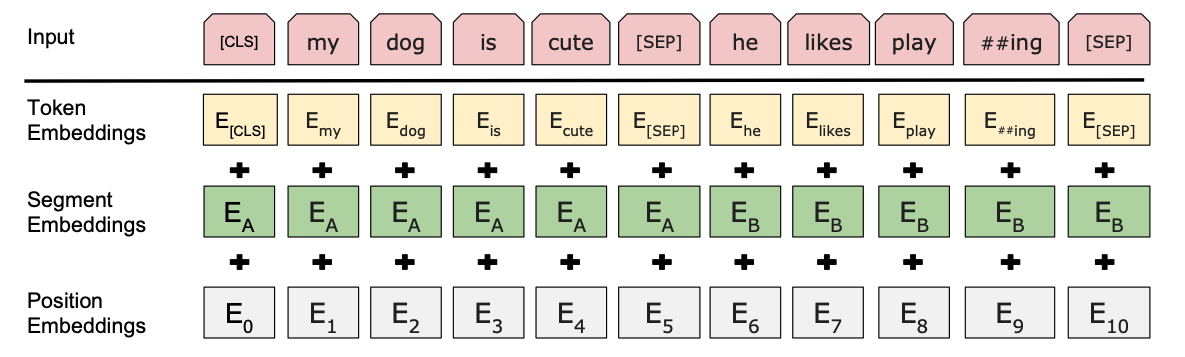
\includegraphics[width=.9\textwidth]{figures/bert}
    \end{figure}
    \vspace{-1em}
    \begin{itemize}[<+->]
        \item Tokenization: wordpiece (similar to byte pair encoding) (see \href{https://huggingface.co/learn/nlp-course/chapter6/6?fw=pt}{details})
        \item \texttt{[CLS]}: first token of all sequences; used for next sentence prediction
        \item Distinguish two sentences in a pair: \texttt{[SEP]} and segment embedding
        \item Learned position embedding
        \item 12 (base; 110M params) or 24 (large; 340M params) layer Transformer
    \end{itemize}
\end{frame}

\begin{frame}
    {Finetuning BERT}
        Classification tasks:
            Add a linear layer (randomly initialized) on top of the \texttt{[CLS]} embedding
            $$
            p(y\mid x) = \mathrm{softmax}(Wh_{\text{[CLS]}}+b)
            $$
            \begin{figure}
                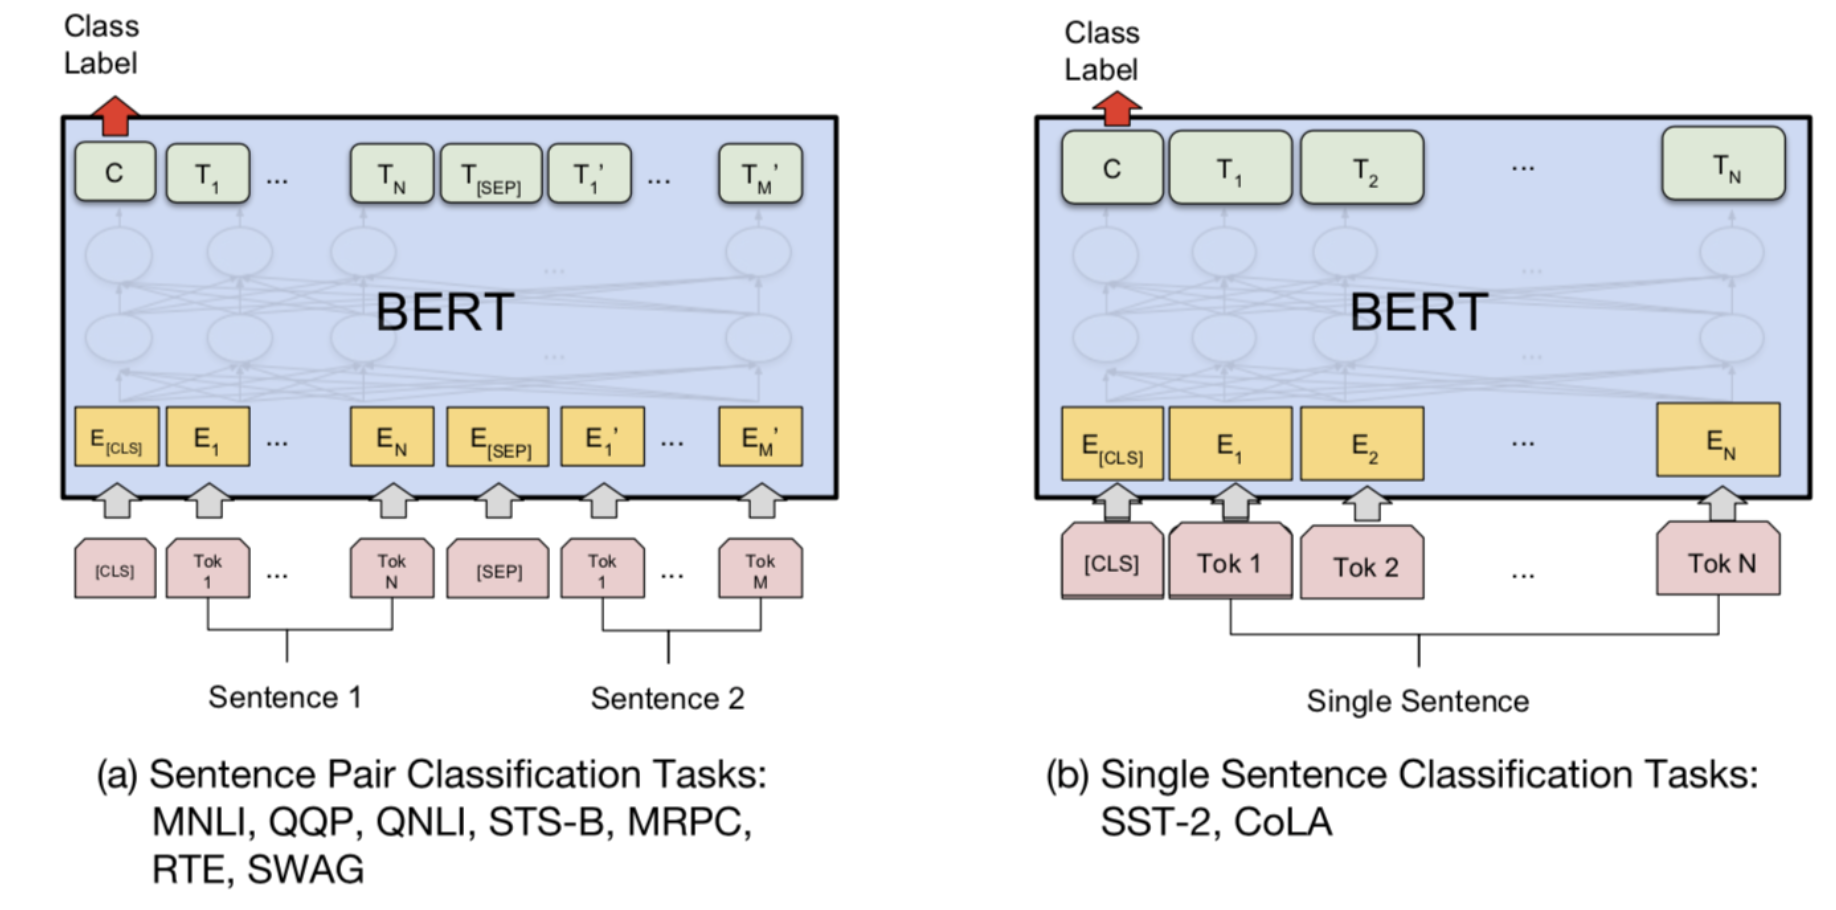
\includegraphics[width=0.8\textwidth]{figures/bert-classification}
            \end{figure}
\end{frame}

\begin{frame}
    {Finetuning BERT}
        Sequence labeling tasks:
            Add linear layers (randomly initialized) on top of every token 
            $$
            p(y_i \mid x) = \mathrm{softmax}(Wh_{i}+b)
            $$
            \begin{figure}
                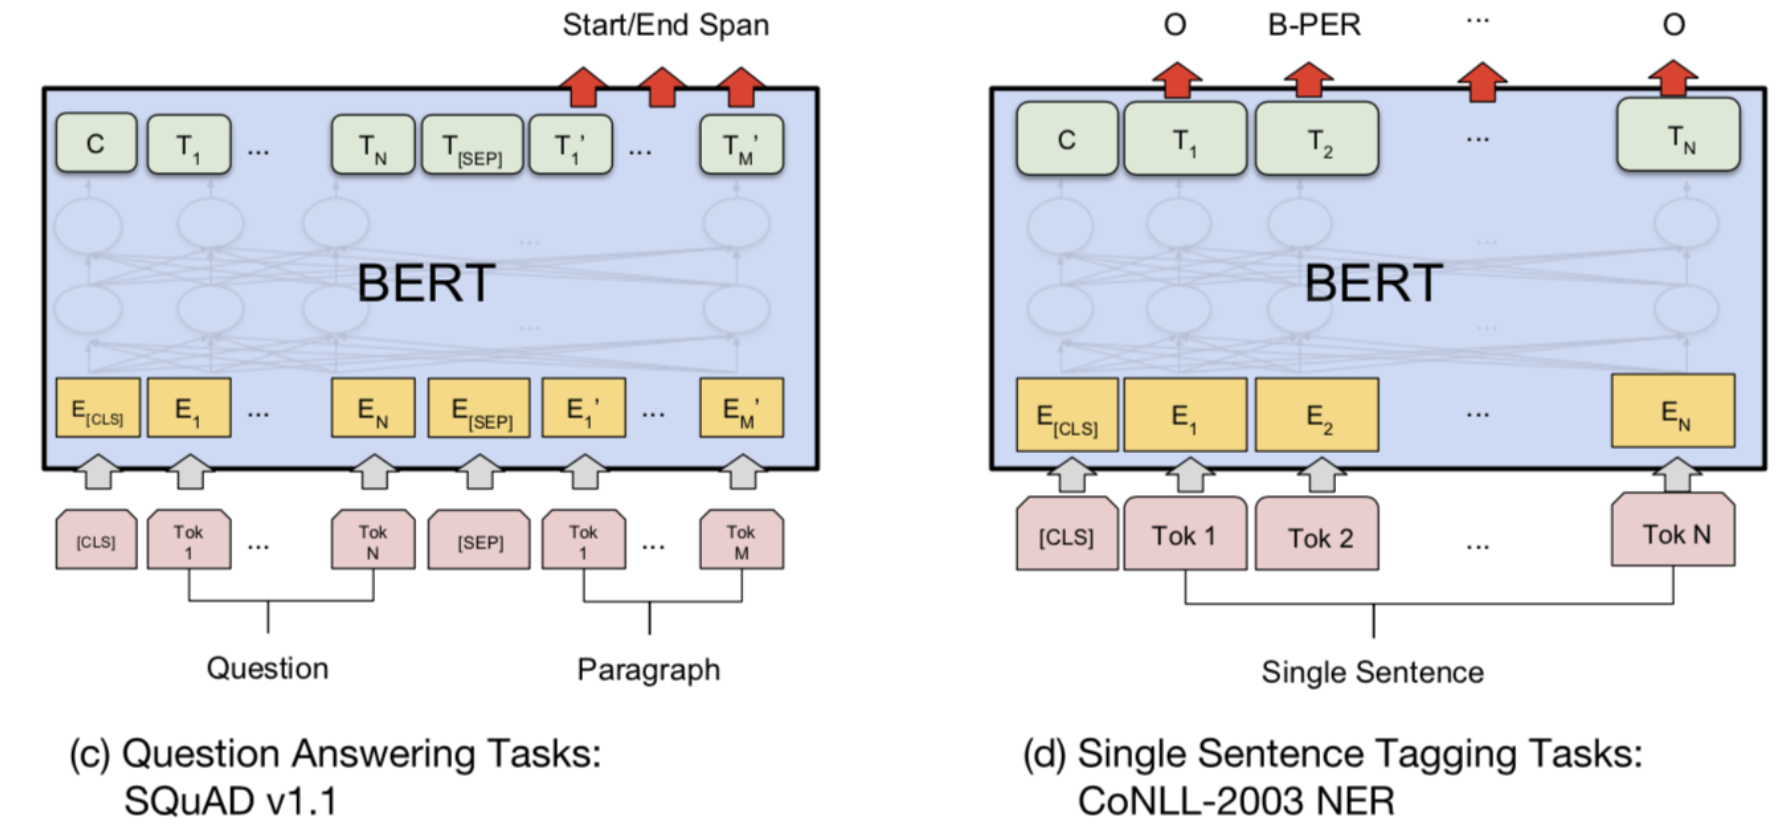
\includegraphics[width=0.8\textwidth]{figures/bert-seq-label}
            \end{figure}
\end{frame}

\begin{frame}
    {Finetuning BERT}

    \begin{itemize}
        \item Finetune all parameters (both the newly added layer and the pretrained weights)
        \item Use a small learning rate (e.g., 1e-5)
        \item Train for a small number of epochs (e.g, 3 epochs)
        \item Led to SOTA results on many NLU tasks
    \end{itemize}
        \think{How to generate text from BERT?} 
\end{frame}

\begin{frame}
    {Encoder-decoder models}

    An encoder-decoder model encodes input text to a sequence of contextualized representations, and decodes a sequence of tokens autoregressively.
    \begin{align*}
        h_1,\ldots,h_n &= \mathrm{Encoder}(x_1,\ldots,x_n) \\
        s_1,\ldots,s_m &= \mathrm{Decoder}(y_0,\ldots,y_{m-1}, h_1,\ldots,h_n)\\
        p(y_i\mid x, y_{<i}) &= \mathrm{softmax}(Ws_i+b)
    \end{align*}

    \pause
    How do we train the encoder-decoder?
    \begin{itemize}
        \item Use any supervised task, e.g., machine translation 
        \item Use self-supervised learning: predict text spans from their context 
    \end{itemize}
\end{frame}

\begin{frame}
    {Masked language modeling using an encoder-decoder}

    \textbf{Input}: text with corrupted spans\\
    \textbf{Output}: recovered spans

    \begin{figure}
        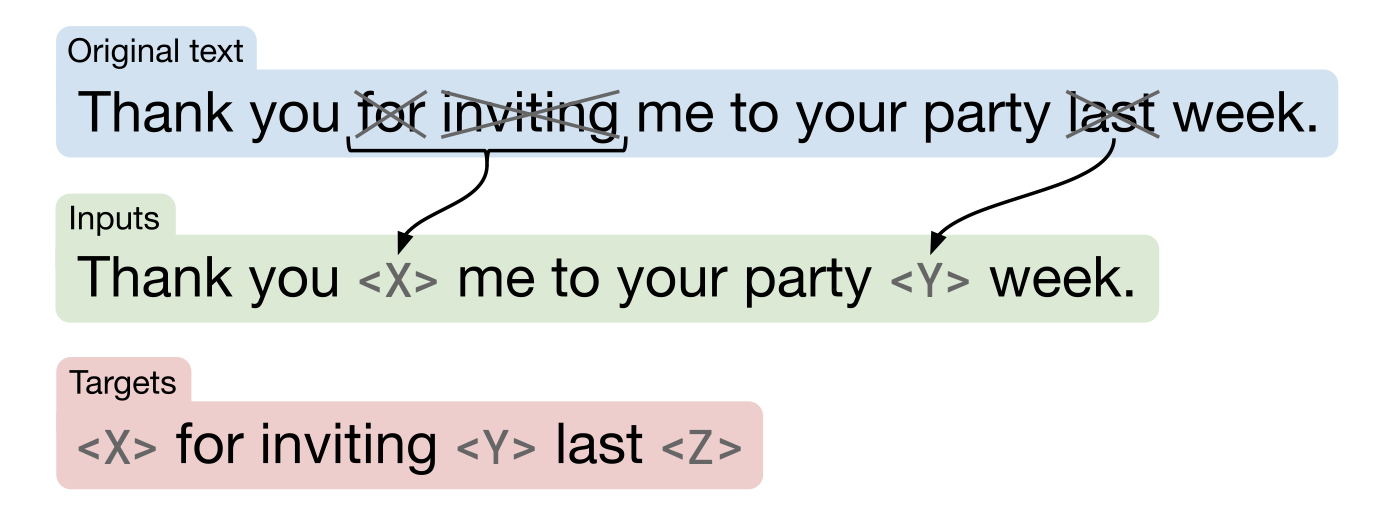
\includegraphics[height=3cm]{figures/t5-span}
    \end{figure}

    Compare with encoder-only models:\\
    \begin{itemize}
        \item Encoder: predict single tokens based on encoder representation
        \item Encoder-decoder: predict a sequence of tokens (flexibility in objective design)
    \end{itemize}
\end{frame}

\begin{frame}
    {T5: objective}

    \begin{itemize}
        \item First train on unlabele data by \textbf{masked language modeling}
            \begin{itemize}
                \item Predict corrupted spans as a sequence
            \end{itemize}
        \item Then \blue{continue training} by \textbf{supervised multitask learning}
            \begin{itemize}
                \item Formulate tasks as text-to-text format using a prefix to denote the task
                \item Mixing examples from different datasets when constructing batches  
            \end{itemize}
    \begin{figure}
        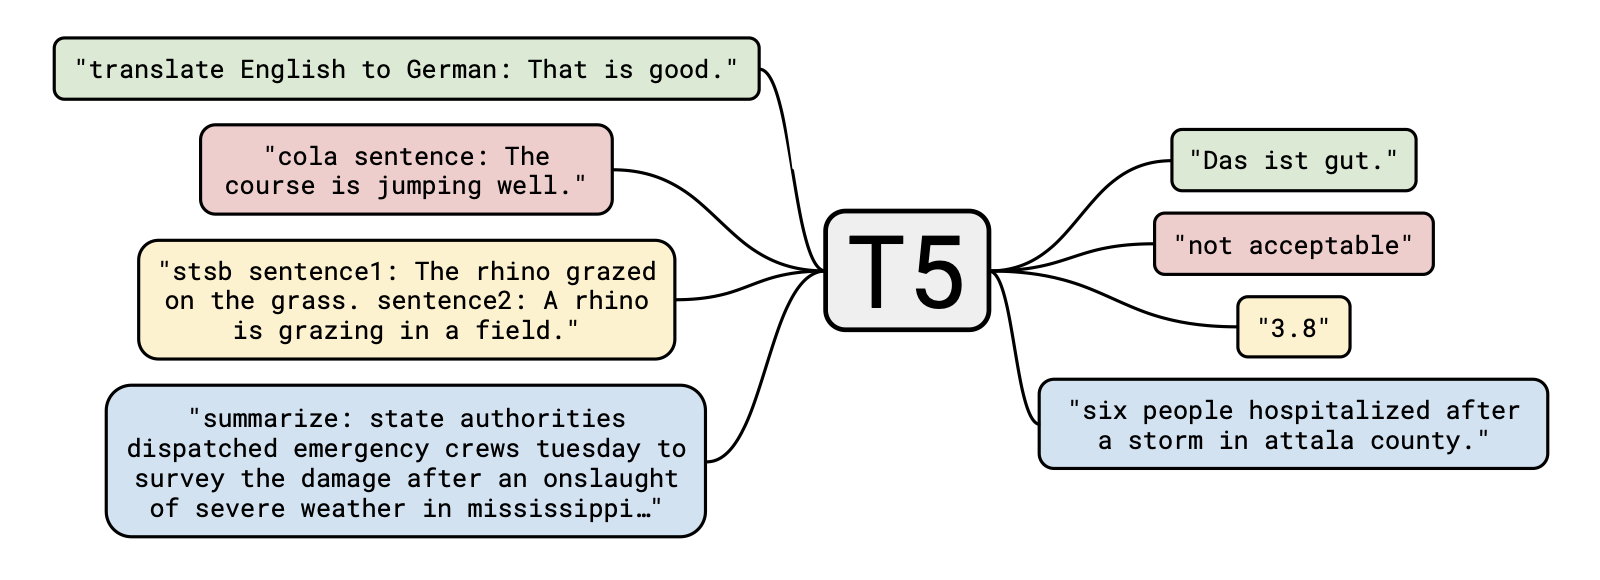
\includegraphics[height=4cm]{figures/t5-mtl}
    \end{figure}
        \item Jointly training with the two objectives works slightly worse
    \end{itemize}
\end{frame}

\begin{frame}
    {T5: finetune}
    \begin{itemize}
        \item Formulate the task in text-to-text format
        \item Fine-tune all parameters (similar to BERT fine-tuning)
        \item Advantages over encoder models: unified modeling of many different tasks including text generation
    \end{itemize}
\end{frame}

\begin{frame}
    {Decoder-only models}

    A decoder-only model predicts the next token given the prefix autoregressively.
    \begin{align*}
        s_1,\ldots,s_m &= \mathrm{Decoder}(y_0,\ldots,y_{m-1}, h_1,\ldots,h_n)\\
        p(y_i\mid y_{<i}) &= \mathrm{softmax}(Ws_i+b)
    \end{align*}
    (A prefix of $y$ can be the input.)
    \begin{figure}
            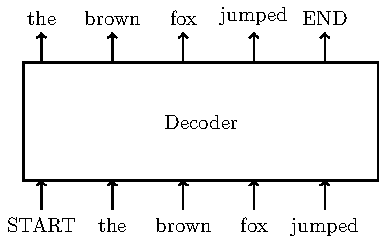
\includegraphics[height=0.5\textheight]{figures/decoder}
    \end{figure}
    (more on language models later)
\end{frame}

\begin{frame}
    {Generative Pretraining (GPT)}
    \begin{itemize}
        \item {\bf Model}: 12 layer decoder-only transformer
        \item {\bf Objective}: next word prediction
            $$
            \max \sum_{y\in\sD} \sum_i \log p(y_i\mid y_{<i})
            $$
        \item {\bf Finetuning}: \blue{auxiliary LM objective} $L_{\text{task}} + \lambda L_{\text{LM}}$ (next word prediction on labeled task data)
    \end{itemize}
\end{frame}

\begin{frame}
    {Generative Pretraining (GPT): task-specific finetuning}
    \begin{figure}
        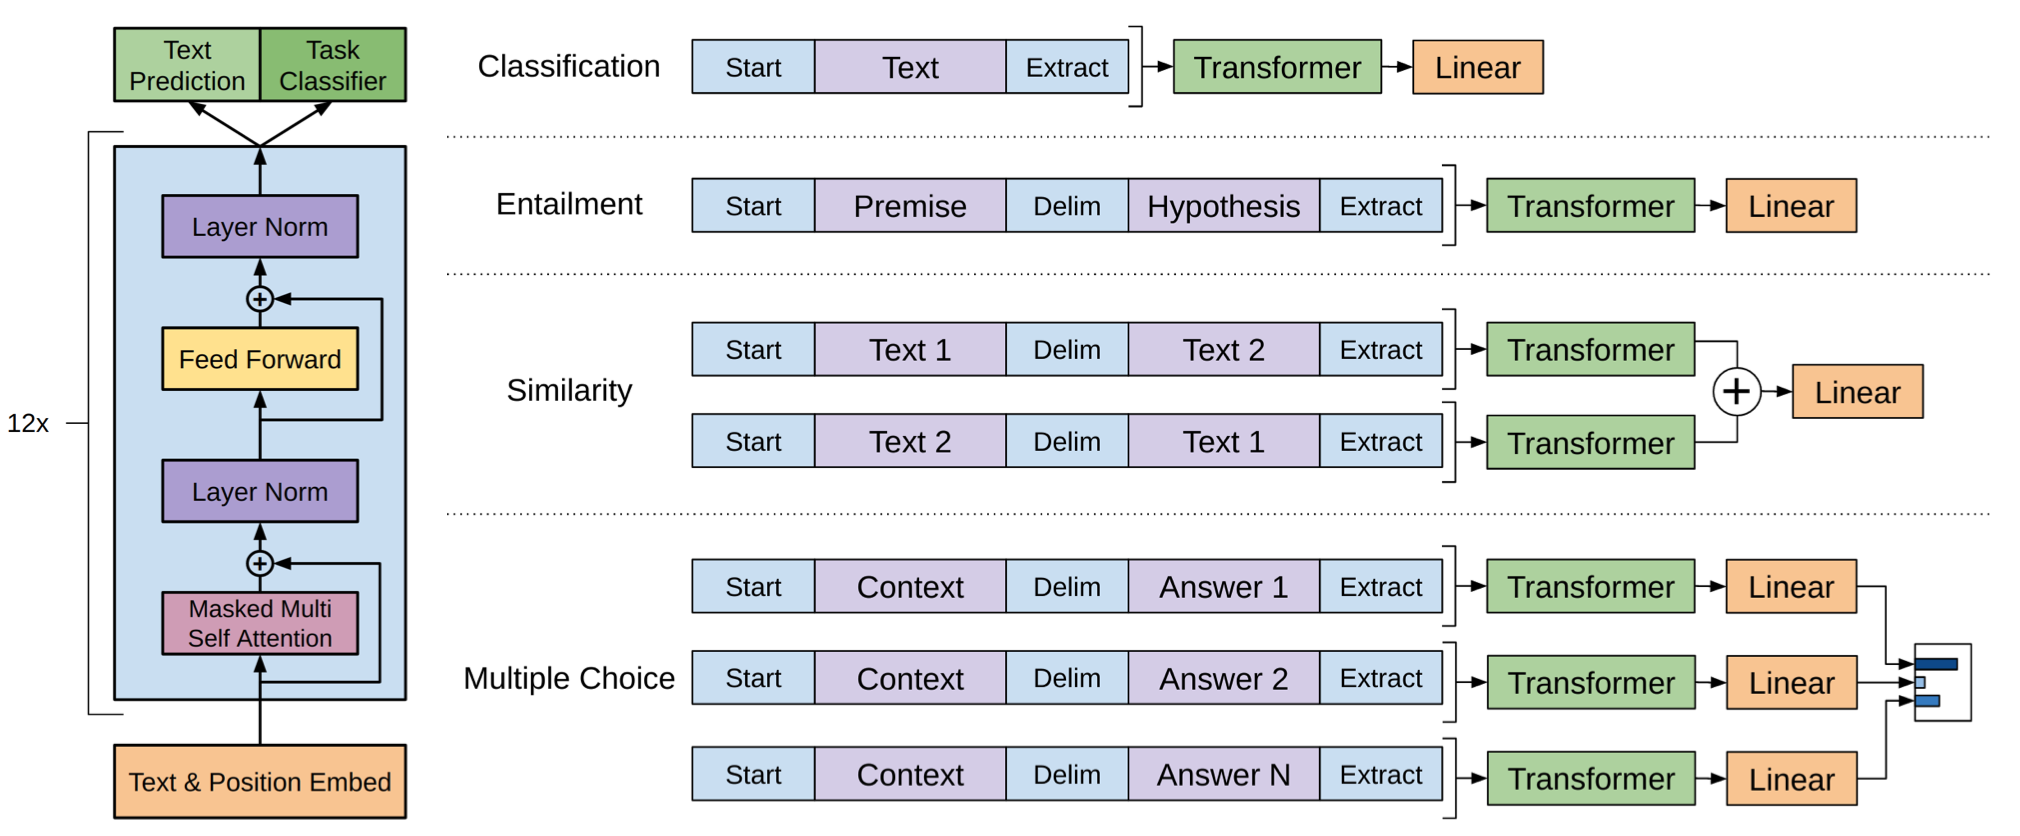
\includegraphics[width=0.9\textwidth]{figures/gpt1}
    \end{figure}
    \begin{itemize}
        \item Single input: linear on top of \texttt{extract}
        \item Multiple input: process each input separately then aggregate
    \end{itemize}
\end{frame}

\begin{frame}
    {Ablation studies of GPT}
    Architecture, pretraining, finetuning: which is critical?
    \begin{figure}
        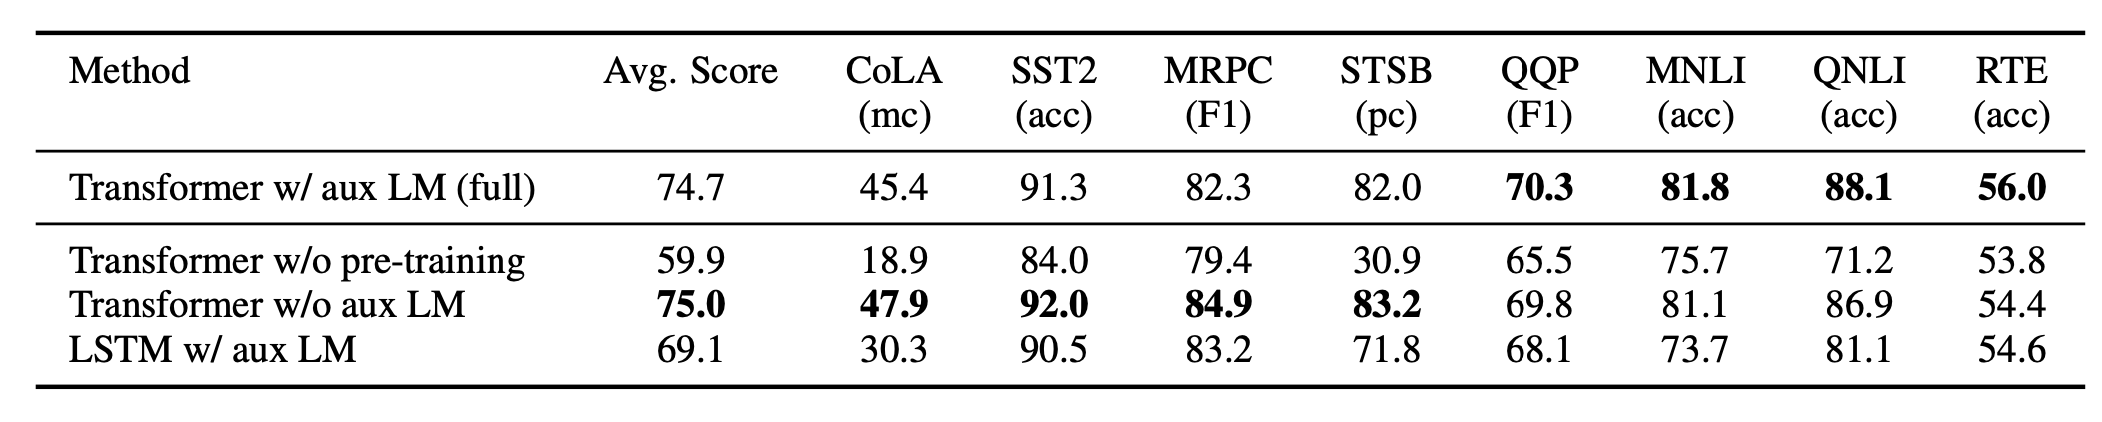
\includegraphics[width=\textwidth]{figures/gpt-ablation}
    \end{figure}
    \begin{itemize}
        \item Auxiliary objective only helps on larger datasets (MNLI, QQP)
        \item Pretrained transformer $>$ pretrained LSTM (single layer) $>$ non-pretrained transformer
    \end{itemize}
\end{frame}

\begin{frame}
    {Compare with BERT}
    \begin{figure}
        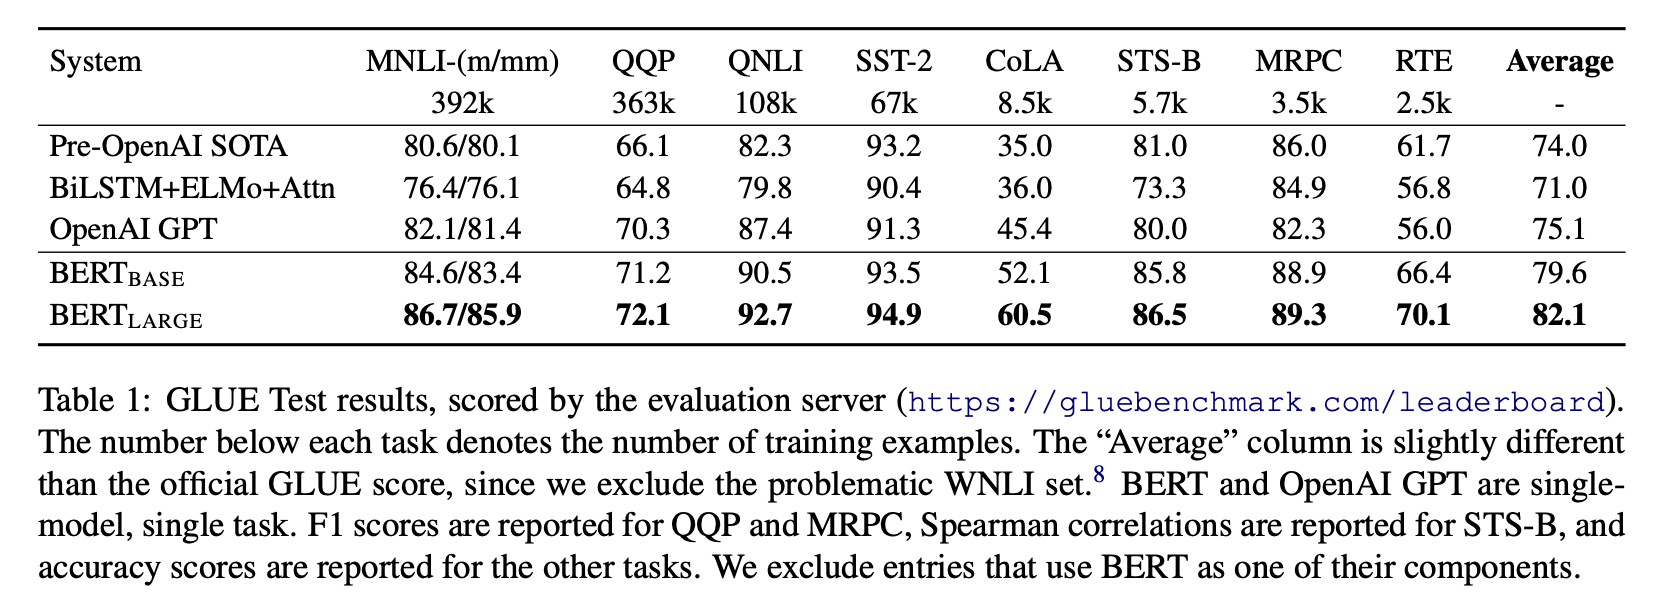
\includegraphics[width=\textwidth]{figures/bert-results}
    \end{figure}
    Medium-sized encoder models tend to work better than decoder-only models when finetuned
\end{frame}

\begin{frame}
    {Encoder-only vs decoder-only models: attention}
    \begin{tikzpicture}
        \node(dec) {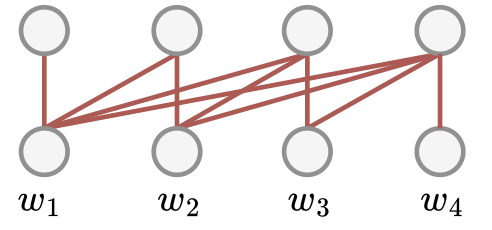
\includegraphics[height=2cm]{figures/dec-attn}};
        \node[above=0.5cm of dec] {Decoder-only};
        \node(enc) [right= of dec]{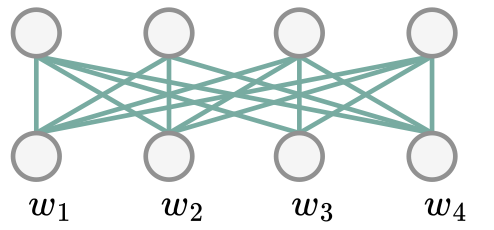
\includegraphics[height=2cm]{figures/enc-attn}};
        \node[above=0.5cm of enc] {Encoder-only};
    \end{tikzpicture}

    \pause
    Encoder-only models provides better embeddings due to bidirectional attention.
\end{frame}

\begin{frame}
    {Encoder-only vs decoder-only models: generation}
    Decoder-only models can make predictions through generation {\em without finetuning}

    \vspace{1em}
    \pause
    \begin{columns}
        \begin{column}{0.4\textwidth}
        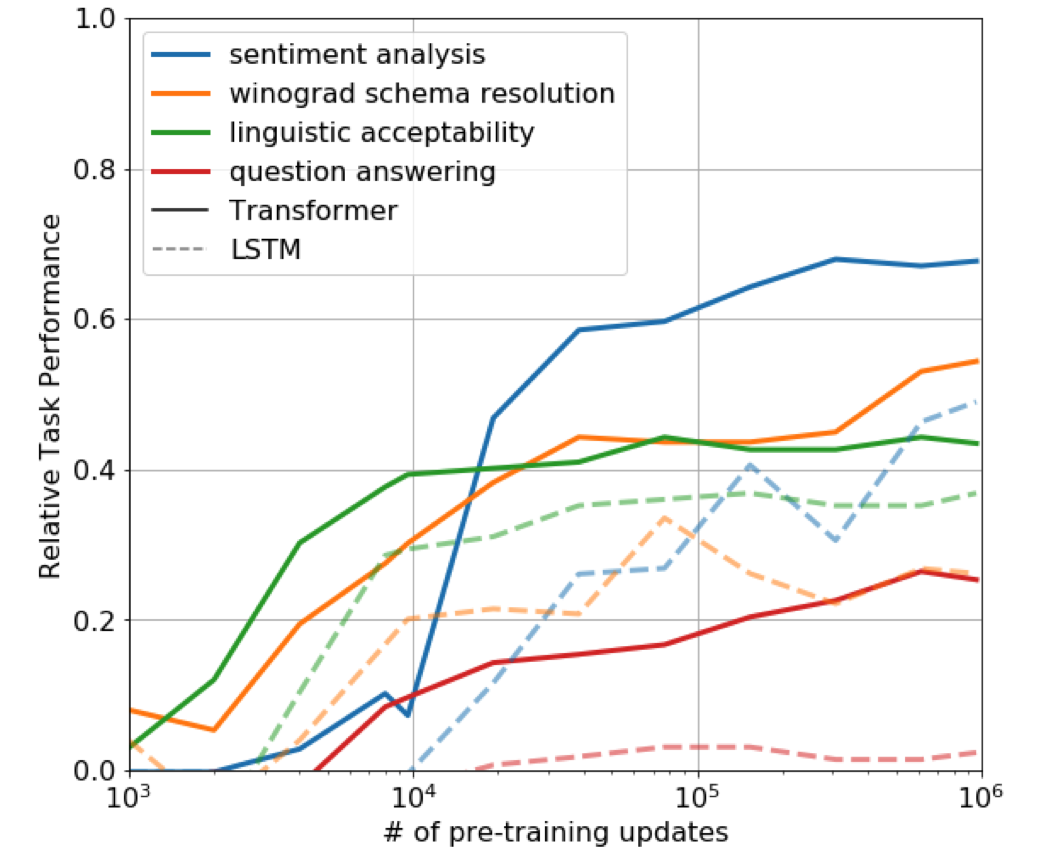
\includegraphics[width=\textwidth]{figures/gpt1-zs}
        \end{column}
        \begin{column}{0.6\textwidth}
            Heuristics for zero-shot prediction:
            \begin{itemize}
                \item Sentiment classification: [example] + very + \{positive, negative\} $\quad$ \blue{\em prompting}
                \item Linguistic acceptability: thresholding on log probabilities
                \item Multiple choice: predicting the answer with the highest log probabilities
            \end{itemize}
            \textbf{Scaling trend}: zero-shot performance increases during pretraining
        \end{column}
    \end{columns}
\end{frame}

\begin{frame}
    {Encoder-only vs decoder-only models: training efficiency}

    On each sequence: 
    \begin{itemize}
        \item Encoder-only models are trained on \blue{15\%} (mask rate) of the tokens
        \item Decoder-only models are trained on \blue{all} tokens 
    \end{itemize}

    \pause
    What about encoder-decoder models?
    \begin{itemize}
        \item Flexibility on encoder design, e.g., full attention on input context
        \item Limited advantage on long-form generation tasks over decoder-only model 
        \item More resource available for decoder-only models 
    \end{itemize}
\end{frame}

% TODO: more on data curation (Olmo, LLM360?)?
%\begin{frame}
%    {What are these models trained on?}
%
%    Both quantity and quality are important
%    \begin{itemize}
%        \item Wikipedia: encyclopedia articles (\green{clean}, \red{single domain})
%        \item Toronto Books Corpus: e-books (\green{diverse domain}) 
%        \item WebText (40GB): content submitted to Reddit with a vote $\ge 3$ (\green{diverse}, \red{bias}) 
%        \item CommonCrawl (20TB): scraped HTML with markers removed (\green{diverse, large}, \red{noisy, bias})
%            \begin{itemize}
%                \item A cleaned version: C4 (750GB)
%            \end{itemize}
%    \end{itemize}
%
%    Active research area: What data is good for pretraining? 
%\end{frame}

\section{Optimization}

\begin{frame}
    {Optimization for pretraining}
    What are challenges of optimization in pretraining?
    \begin{wideitemize}
        \item Numerical stability (no NaN and diverging losses)\\
            \gray{initialization, normalization, learning rate schedule}
        \item Memory efficiency (work with billions of parameters)\\
            \gray{mixed precision, gradient accumulation}
    \end{wideitemize}
\end{frame}

\begin{frame}
    {Adam optimizer}

    {\bf Key ideas}:\\
    \begin{wideitemize}
        \item Momentum
            \begin{itemize}
                \item Motivation: having an inertia of moving in the same direction $\rightarrow$ reduce oscillation
                \item How: maintain a "memory" (moving average) of past updates
            \end{itemize}
        \pause
        \item Adaptive step size for each parameter
            \begin{itemize}
                \item Intuition:\\
                    flat regions (gradient changing slowly) $\rightarrow$ take larger steps\\
                    steep regions (gradient changing fast) $\rightarrow$ take smaller steps\\
                \item Handle sparse features well (e.g., rare words embeddings aren't updated often)
            \end{itemize}
    \end{wideitemize}
\end{frame}

\begin{frame}
    {Adam optimizer}
    \begin{itemize}[<+->]
        \item Compute gradient $g_t$
        \item Update first order moments (mean)
    \begin{equation}
            m_t = \beta_1 m_{t-1} + (1 - \beta_1) g_t
        \end{equation}
    \item Update second order moments (variance)
        \begin{equation}
            v_t = \beta_2 v_{t-1} + (1 - \beta_2) g_t^2
        \end{equation}
    \item Correct bias in moment estimates
        \begin{equation}
            \hat{m}_t = \frac{m_t}{1 - \beta_1^t}, \quad \hat{v}_t = \frac{v_t}{1 - \beta_2^t}
        \end{equation}
    \item Update parameters
        \begin{equation}
            \theta_t = \theta_{t-1} - \eta \frac{\hat{m}_t}{\sqrt{\hat{v}_t} + \epsilon}
        \end{equation}
    \end{itemize}
    \pause
    \think{What is the memory cost of SGD vs Adam?}
\end{frame}

\begin{frame}
    {Learning rate schedule}
    \begin{wideitemize}
        \item {\bf Warmup}: don't want to start with large learning rate for stability
        \item {\bf Decay}: reducing learning rate as model converges\\
            linear (used by BERT), cosine, exponential
    \end{wideitemize}
    \begin{figure}
        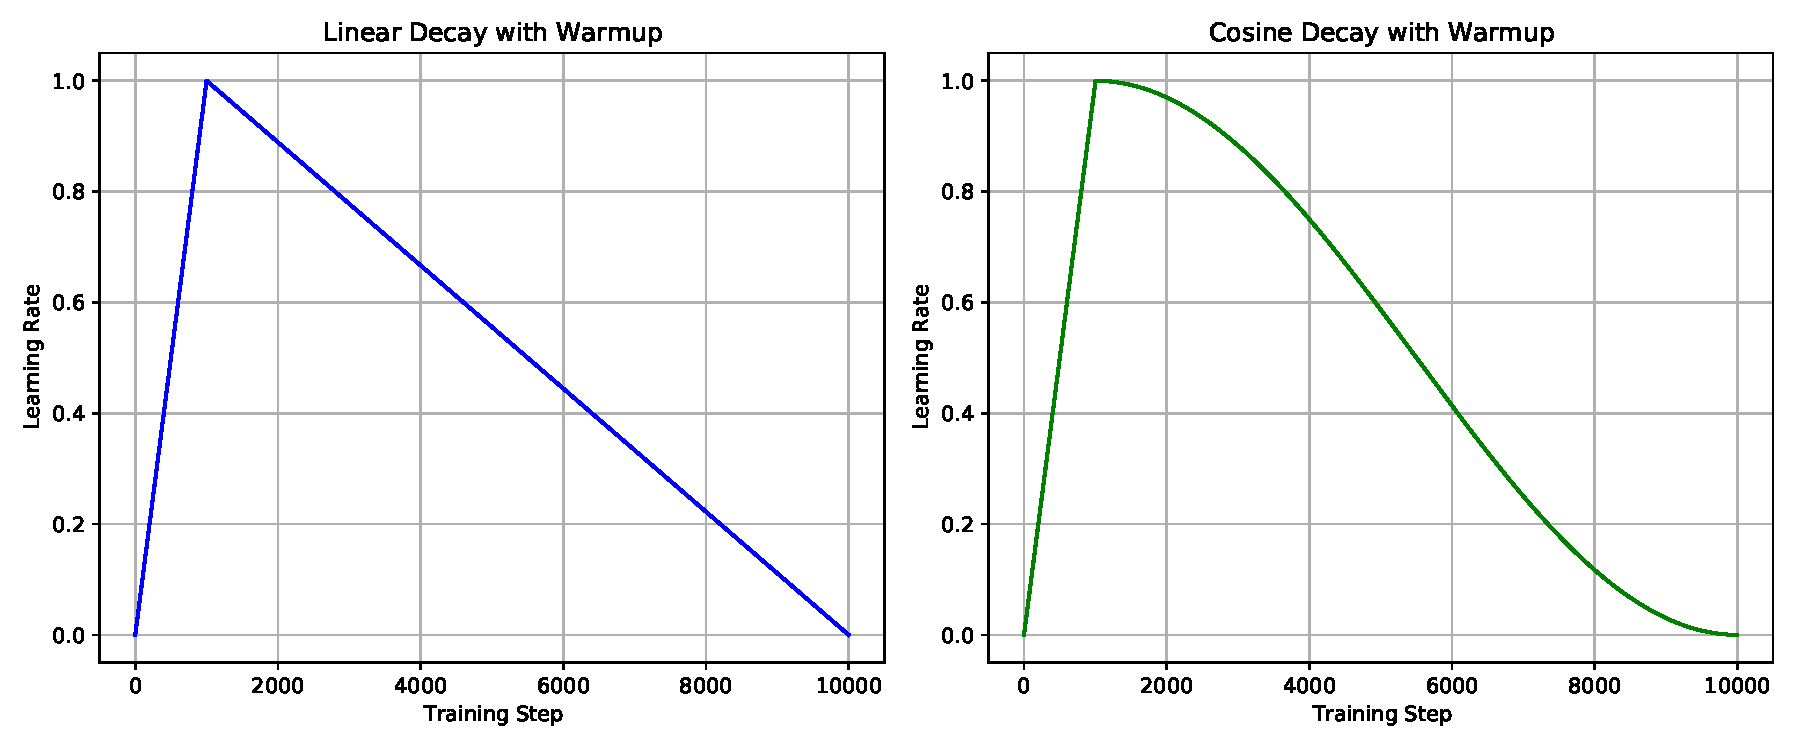
\includegraphics[width=0.7\textwidth]{figures/learning-rate}
    \end{figure}
\end{frame}

\begin{frame}
    {Gradient accumulation}
    Simulate large batch training with limited GPU memory
    \begin{figure}
        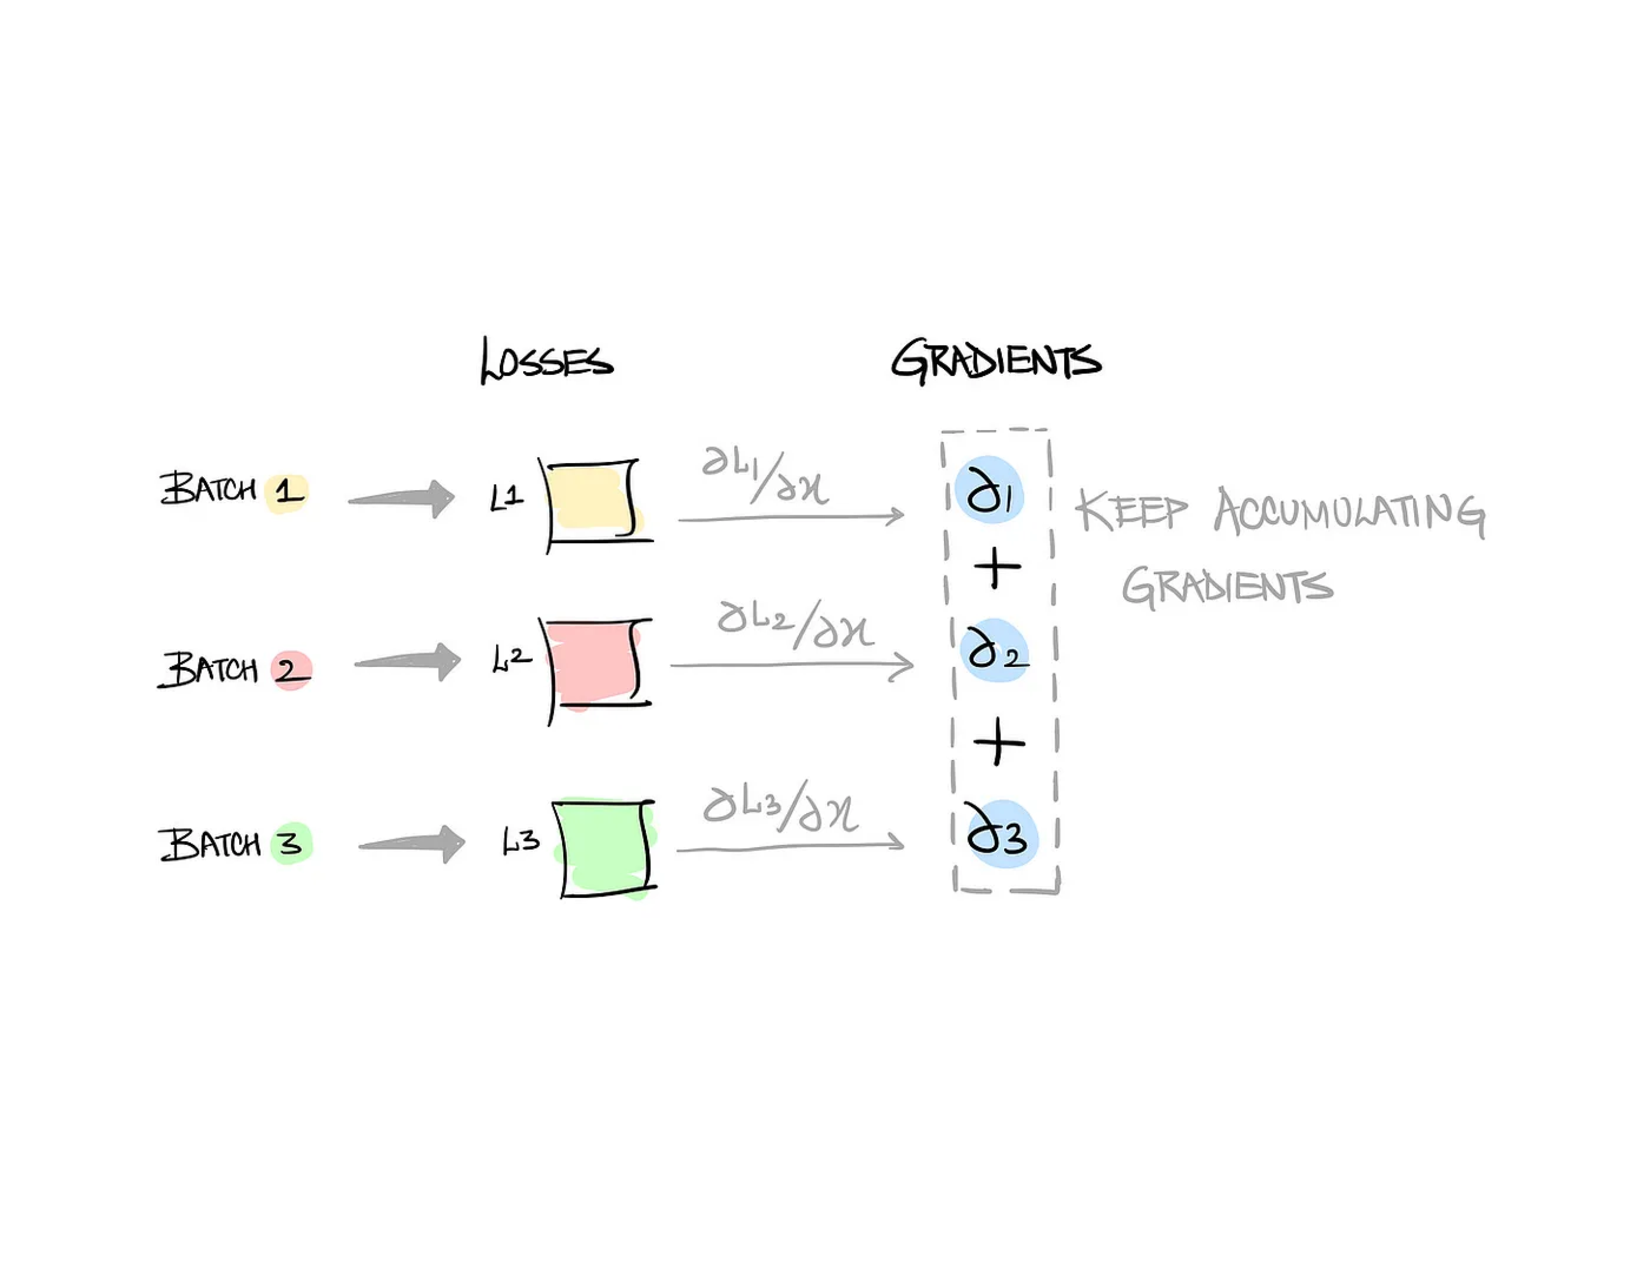
\includegraphics[width=0.7\textwidth]{figures/grad-accum}
        \caption{From \href{https://medium.com/@harshit158/gradient-accumulation-307de7599e87}{Harshit Sharma}}
    \end{figure}
\end{frame}

\end{document}
